\documentclass[12pt]{article}
\setlength{\oddsidemargin}{0.25 in}
\setlength{\evensidemargin}{-0.25 in}
\setlength{\topmargin}{-0.6 in}
\setlength{\textwidth}{6.5 in}
\setlength{\textheight}{8.5 in}
\setlength{\headsep}{0.75 in}
\setlength{\parindent}{0 in}
\setlength{\parskip}{0.1 in}

%
% ADD PACKAGES here:
%

\usepackage{amsmath,amsfonts,amssymb,graphicx,mathtools}
\usepackage{multirow,url}

%
% The following commands set up the lecnum (lecture number)
% counter and make various numbering schemes work relative
% to the lecture number.
%
\newcounter{lecnum}
\renewcommand{\thepage}{\thelecnum-\arabic{page}}
\renewcommand{\thesection}{\thelecnum.\arabic{section}}
\renewcommand{\theequation}{\thelecnum.\arabic{equation}}
\renewcommand{\thefigure}{\thelecnum.\arabic{figure}}
\renewcommand{\thetable}{\thelecnum.\arabic{table}}

%
% The following macro is used to generate the header.
%
\newcommand{\lecture}[4]{
   \pagestyle{myheadings}
   \thispagestyle{plain}
   \newpage
   \setcounter{lecnum}{#1}
   \setcounter{page}{1}
   \noindent
   \begin{center}
   	\framebox{
   		\vbox{\vspace{2mm}
   			\hbox to 6.28in { {\bf MATH 254: Introduction to Statistics
   					\hfill #3} }
   			\vspace{4mm}
   			\hbox to 6.28in { {\Large \hfill Lesson #1: #2  \hfill} }
   			\vspace{2mm}
   			\hbox to 6.28in { {\hfill Corresponding Workbook Module: #4} }
   			\vspace{2mm}}
   	}
   \end{center}
   \markboth{Handout #1}{Handout #1}

   %{\bf Note}: {\it LaTeX template courtesy of UC Berkeley EECS dept.}

   %{\bf Disclaimer}: {\it These notes have not been subjected to the usual scrutiny reserved for formal publications.  They may be distributed outside this class only with the permission of the instructor.}
   %\vspace*{4mm}
   \vspace*{-4mm}
}
%
% Convention for citations is authors' initials followed by the year.
% For example, to cite a paper by Leighton and Maggs you would type
% \cite{LM89}, and to cite a paper by Strassen you would type \cite{S69}.
% (To avoid bibliography problems, for now we redefine the \cite command.)
% Also commands that create a suitable format for the reference list.
\renewcommand{\cite}[1]{[#1]}
\def\beginrefs{\begin{list}%
        {[\arabic{equation}]}{\usecounter{equation}
         \setlength{\leftmargin}{2.0truecm}\setlength{\labelsep}{0.4truecm}%
         \setlength{\labelwidth}{1.6truecm}}}
\def\endrefs{\end{list}}
\def\bibentry#1{\item[\hbox{[#1]}]}

%Use this command for a figure; it puts a figure in wherever you want it.
%usage: \fig{NUMBER}{SPACE-IN-INCHES}{CAPTION}
\newcommand{\fig}[3]{
			\vspace{#2}
			\begin{center}
			Figure \thelecnum.#1:~#3
			\end{center}
	}
% Use these for theorems, lemmas, proofs, etc.
\newtheorem{example}{Example}[lecnum]
\newtheorem{exercise}{Exercise}[lecnum]

\newtheorem{theorem}{Theorem}[lecnum]
\newtheorem{definition}[theorem]{Definition}
\newenvironment{proof}{{\bf Proof:}}{\hfill\rule{2mm}{2mm}}

% **** IF YOU WANT TO DEFINE ADDITIONAL MACROS FOR YOURSELF, PUT THEM HERE:

\newcommand\E{\mathbb{E}}

\begin{document}
%FILL IN THE RIGHT INFO.
%\lecture{**LECTURE-NUMBER**}{**DATE**}{**LECTURER**}{**SCRIBE**}
\lecture{1}{Describing Data}{Mintaek Lee}{1}
%\footnotetext{These notes are partially based on those of Nigel Mansell.}

% **** YOUR NOTES GO HERE:
\begin{example}
	Mintaek is interested in how many geese are in Julia Davis Park. Mintaek sits on a bench from 9 am to 9 pm and counts the number of geese he observes. He repeated it for 10 consecutive days. Mintaek’s geese counts of the day are listed below.
	\[ 20 \quad 24 \quad 24 \quad 24 \quad 24 \quad 26 \quad 28 \quad 28 \quad 28 \quad 29 \]
\end{example}

\textit{\textbf{Part A.} Find mean, median, and standard deviation of the given data set.}

\textbf{Solution}: We can find the sample mean as
\[ \bar{x} = \dfrac{1}{n} \sum_{i=1}^{n} x_i = \dfrac{20+24+24+24+24+26+28+28+28+29}{10} = \dfrac{255}{10} = 25.5 \]

There are 10 observations. Since $n=10$ is an even number, the median is the average of two middle observations, 24 and 26. Therefore, median is $\dfrac{24+26}{2} = 25$. If $n$ were an odd number, the median would have been the middle observation.

We can find the standard deviation using the following procedure (proceed from left to right)
\begin{table}[h]
	\centering
	\begin{tabular}{cccc|c}
		$x$ & $-\bar{x}$ & $(x-\bar{x})$ & $(x-\bar{x})^2$ & $\sum (x-\bar{x})^2$ \\ \hline
		$20$ & $-25.5$ & $-5.5$ & $30.25$ & $70.5$ \\
		$24$ & $-25.5$ & $-1.5$ & $\phantom{0}2.25$ &  \\
		$24$ & $-25.5$ & $-1.5$ & $\phantom{0}2.25$ &  \\
		$24$ & $-25.5$ & $-1.5$ & $\phantom{0}2.25$ &  \\
		$24$ & $-25.5$ & $-1.5$ & $\phantom{0}2.25$ &  \\
		$26$ & $-25.5$ & $+0.5$ & $\phantom{0}0.25$ &  \\
		$28$ & $-25.5$ & $+2.5$ & $\phantom{0}6.25$ &  \\
		$28$ & $-25.5$ & $+2.5$ & $\phantom{0}6.25$ &  \\
		$28$ & $-25.5$ & $+2.5$ & $\phantom{0}6.25$ &  \\
		$29$ & $-25.5$ & $+3.5$ & $12.25$ & 
	\end{tabular}
\end{table}

So we get $s = \sqrt{\dfrac{1}{n-1} \sum_{i=1}^{n} (x_i-\bar{x})^2} = \sqrt{ \dfrac{1}{10-1} \times 70.5} = \sqrt{\dfrac{70.5}{9}} = 2.7988$.

\pagebreak

\textit{\textbf{Part B.} Make stem-and-leaf plot and histogram of the data.}

\textbf{Solution}: Stem-and-leaf plot is shown below.

\begin{tabular}{l|ll}
	$2$ & $0$       & \hspace{1 cm} Stem: tens digit\\
	$2$ &    		& \hspace{1 cm} Leaf: ones digit\\
	$2$ & $4444$  	& \\
	$2$ & $6$		 & \hspace{1 cm} Key: $2|4=24$\\
	$2$ & $8889$  &
\end{tabular}
	
Frequency table and the histogram are shown below.

\begin{minipage}{0.49\textwidth}
	\def\arraystretch{1.2}
	\begin{tabular}{l|l}
		Intervals & Frequency  \\ \hline
		$[20,22)$ & 1 \\
		$[22,24)$ & 0 \\
		$[24,26)$ & 4 \\
		$[26,28)$ & 1 \\
		$[28,30)$ & 4
	\end{tabular}
\end{minipage}
\begin{minipage}{0.49\textwidth}
	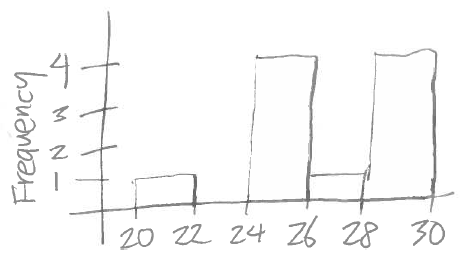
\includegraphics[width=7cm]{Figures/fig7.png}
\end{minipage}

For more information on how to make stem-and-leaf plots and histograms, review the videos for pre-class reading or Section 1.2 of your textbook.

\textit{\textbf{Part C.} Find the five number summary of the given data set. Are there any outliers?}

\textbf{Solution}: We found median as 25 from Part A. We also find minimum as 20 and maximum as 29. To find the five number summary, we need first quartile $(Q_1)$ and third quartile $(Q_3)$.

First quartile $(Q_1)$ is the median of the values below (lower than) the median of the entire data set. Median was 25. Values below the median were: 20, 24, 24, 24, 24. Since there are five of them, the median of those five values would just be the middle value, which is 24.

Third quartile $(Q_3)$ is the median of the values above (higher than) the median of the entire data set. Median was 25. Values above the median were: 26, 28, 28, 28, 29. Since there are five of them, the median of those five values would just be the middle value, which is 28.

The five number summary is then:
\begin{tabular}{lllll}
	Min & $Q_1$ & Median & $Q_3$ & Max \\
	20  & 24      & 25     & 28      & 29
\end{tabular}

To determine if there are any outliers, we use the following procedure
\begin{align*}
	&Q_1 - 1.5 \times IQR = 24 - 1.5 \times 4 = 24 - 6 = 18 \\
	&Q_3 + 1.5 \times IQR = 28 + 1.5 \times 4 = 28 + 6 = 34
\end{align*}
since $IQR = Q_3 - Q_1 = 28 - 24 = 4$.

We check if any observations fall outside the interval $(Q_1 - 1.5 \times IQR, Q_3 + 1.5 \times IQR) = (18, 34)$. Since no observation fall outside $(18,34)$, we determine that there are no outliers.

\textit{\textbf{Part D.} Make a boxplot of the given data set.}

\textbf{Solution}: 

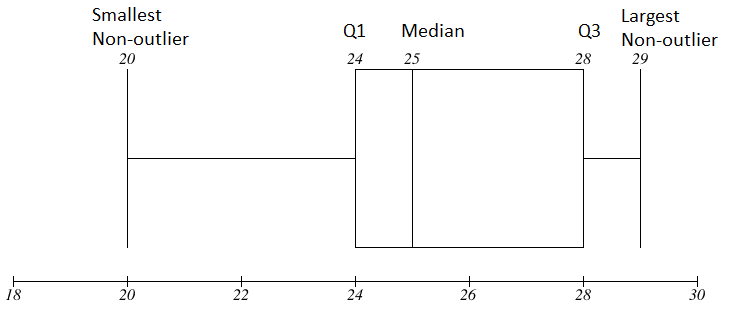
\includegraphics[width=12cm]{Figures/fig8.png}

For more information on how to make boxplots, see workbook page 16.

\textit{\textbf{Part E.} Fully describe the distribution of Mintaek's geese counts.}

\textbf{Solution}: When describing the distribution of a given data set, researchers generally focus on the four elements: center, unusual features, spread, and shape. The acronym ``\textbf{CUSS}'' may help you remember those four features. For more information, see workbook page 11.

What we found so far about this data set are as follows:
\begin{itemize}
	\item \textbf{C}enter: mean was 25.5 and median was 25
	\item \textbf{U}nusual features: There are no outliers, although there is a gap between 20 and 24.
	\item \textbf{S}pread: sample standard deviation was 2.7988 and IQR was 4. Or the five number summary was 20, 24, 25, 28, 29.
	\item \textbf{S}hape: The distribution appears to be bimodal with slight left-skew.
\end{itemize}

In most cases, you need not list all findings. General rule of thumb is that mean and standard deviation are preferred when the data appear symmetric, and median and IQR (or five number summary) are preferred when the data appear skewed.

For this data set, you could say
\begin{quote}
	Median is 25. 
	
	There are no outliers, although there is a gap between 20 and 24. 
	
	IQR is 4 (OR five number summary is  20, 24, 25, 28, 29). 
	
	The distribution appears to be bimodal with slight left-skew.
\end{quote}
Note that it is unnecessary to write out CUSS.

\pagebreak

\begin{example}
	Suppose that weights of adult emperor penguins are approximately normally distributed with mean 75 lbs and standard deviation 15 cm.	
\end{example}

\textit{\textbf{Part A.} Mintaek is interested in adopting a pet emperor penguin. Mintaek found an emperor penguin weighing 65 lbs. Find a proportion of all penguins weighing less than 65 lbs.}

\textbf{Solution}: Let $X$ be weight of penguins, then $X \sim N(\mu = 75, \sigma = 15)$. We first find the z-score of 65 lbs which is
\[ z = \dfrac{x - \mu}{\sigma} = \dfrac{65 - 75}{15} = -0.67 \]

Since we want to find a proportion of all penguins weighing \textbf{less than} 65 lbs, we want the area under the standard normal curve to the \textbf{left} of $z = -0.67$. Using the standard normal distribution (z) table, we find 0.2514 as the desired area. 

Therefore, 25.14\% of all emperor penguins would weigh less than 65 lbs. In other words, a weight of 65 lbs is about the 25-th percentile of all emperor penguin weights.

\textit{\textbf{Part B.} Mintaek found another emperor penguin. This time, weighing 70 lbs. Find a proportion of all penguins weighing more than 70 lbs.}

\textbf{Solution}: We first find the z-score of 70 lbs which is
\[ z = \dfrac{x - \mu}{\sigma} = \dfrac{70 - 75}{15} = -0.33 \]

Since we want to find a proportion of all penguins weighing \textbf{more than} 70 lbs, we want the area under the standard normal curve to the \textbf{right} of $z = -0.33$. Remember that the standard normal distribution (z) table gives you the area under the standard normal curve to the \textbf{left} of $z = -0.33$ which was found as 0.3707. To find the area under the standard normal curve to the \textbf{right} of $z = -0.33$, we subtract 0.3707 from 1. We find $1 - 0.3707 = 0.6293$ as the desired area. 

Therefore, 62.93\% of all emperor penguins would weigh more than 70 lbs.

\textit{\textbf{Part C.} Find a proportion of all penguins weighing between 65 lbs and 70 lbs.}

\textbf{Solution}: From Part A, we found the area under the standard normal curve to the \textbf{left} of $z = -0.67$ as 0.2504. It means 25.04\% of all emperor penguins would weigh less than 65 lbs.

From Part B, we found the area under the standard normal curve to the \textbf{left} of $z = -0.33$ as 0.3707. It means 37.07\% of all emperor penguins would weigh less than 70 lbs.

To find a proportion of all penguins weighing between 65 lbs and 70 lbs, we subtract 25.04\% from 37.07\%, giving us $37.07\% - 25.14\% = 11.93\%$.

Therefore, 11.93\% of all emperor penguins would weigh between 65 lbs and 70 lbs.

\textit{\textbf{Part D.} Suppose there is a regulation prohibiting Mintaek from adopting a pet emperor penguin whose weight is more than the 70-th percentile. What is the maximum weight of a penguin that Mintaek can legally adopt?}

\textbf{Solution}: The heaviest penguin that Mintaek can legally adopt would have a weight in the 70-th percentile of all emperor weights. It means we will need to find a z-score such that the area under the standard normal curve to the \textbf{left} of it is 0.7. 

Looking at the standard normal distribution (z) table, we find that $z = 0.52$ gives 0.6985 and $z = 0.53$ gives 0.7019. We can make a guess that $z = \frac{0.52 + 0.53}{2} = 0.525$ would give about 0.7 as the area under the standard normal curve to the \textbf{left} of it.

To find the weight $x$ corresponding to the z-score $z = 0.525$, we set up our equation as
\[ z = \dfrac{x - \mu}{\sigma} \implies 0.525 = \dfrac{x - 75}{15} \]

Solving for $x$ gives us $x = 82.875$.

The heaviest penguin that Mintaek can legally adopt would have a weight of 82.875 lbs.

Note that you can still earn full credits even if you used $z = 0.52$ or $z = 0.53$.

\textbf{Additional Comments}: When answering these types of questions, draw the standard normal distribution curve and shade the area you need and areas you find from the table. This practice should help you significantly reduce mistakes.
	
\end{document}